% !TeX spellcheck = en_US
% !TeX encoding = UTF-8
\chapter{Theoretical foundation}

\section{Stress Framework/Biosignals}
\subsection{Photoplethysmogram-PPG}
\subsection{Electrodermal Activity-EDA}
\subsection{Motion Capture}

\LaTeX packages and compilers have the advantage that they can be installed completely independently of the latex editor.
They are summarized in so-called latex distributions.
Recommended distributions on Windows are MikTeX (\href{http://miktex.org/}{http://miktex.org/}) and on OS~X MacTeX \href{https://tug.org/mactex/}{https://tug.org/mactex/}.

The choice of latex editor is usually based on individual needs and tastes.
A recommended, cross-platform editor is TeXstudio \href{http://texstudio.sourceforge.net/}{http://texstudio.sourceforge.net/}.
This offers, among other things, the possibility to display desired positions of the PDF preview directly in the source text.
Another popular editor is TeXnicCenter (\href{http://www.texniccenter.org/}{http://www.texniccenter.org/}).

Finally, the author chooses between the Latex- (PS/Dvi) and the pdflatex compiler.
The respective selection are made in the settings of the editor. \\

Pdflatex:
\begin{itemize}
	\item More advanced than latex
	\item Supports the following image file types: PDF (Vector), PNG, JPG.
	\item Supports EPS images with the package "`epstopdf"' (already included).
	\item Not compatible with old packages that only work with PostScript files.
\end{itemize}

Latex (PS/Dvi):
\begin{itemize}
	\item Works with "`psfrag"' and other PS based packages.
	\item Supports EPS images only without further conversion.
	\item Longer compile time
\end{itemize}65


\section{Robot Collision Avoidance}
\section{Machine Learning Methods}
Insert a table next to a figure taking into account the associated directories (tables, figures):
\begin{figure}[htbp]
%
	\begin{minipage}[t]{0.45\textwidth}
	\centering
	\raisebox{2.5cm}{ %per hand
		\begin{tabular}{cc}
		\toprule
		Configuration & Parameter set \\
		\midrule
		$1$ & $\{p_{1}, \: p_{2}, \: p_{5}\}$ \\
		$2$ & $\{p_{1}, \: p_{4}, \: p_{5}\}$ \\
		$3$ & $\{p_{2}, \: p_{3}, \: p_{4}\}$ \\
		\bottomrule
		\end{tabular}
	}
	\captionof{table}{Definition range of parameters for optimization.} %ins tabellenverzeichnis einfügen
	\label{tab:bsp2}
	\end{minipage}
%
	\begin{minipage}[t]{0.45\textwidth}
	\centering
	  
\includegraphics[width=\textwidth]{images/logos/tud_logo_rgb}
  	\captionof{figure}{Sample diagram}
	\end{minipage}
\end{figure}

%\section{Subcaption: Picture besides picture and table besides table}

The \textit{Subcaption} package (labeling of tables and figures with a), b), ...) should only be chosen if the associated tables/figures really belong together contextually.

\begin{figure}[htbp]
        \centering
        \begin{subfigure}[b]{0.3\textwidth}
        		\centering
                
\includegraphics[width=\textwidth]{images/logos/tud_logo_rgb} 
                \caption{TU Dortmund Logo}
                \label{fig:subfigure_tud_logo}
        \end{subfigure}%
        \quad %add desired spacing between images, e. g. ~, \quad, \qquad, \hfill etc.
          %(or a blank line to force the subfigure onto a new line)
        \begin{subfigure}[b]{0.3\textwidth}
        		\centering
                
\includegraphics[width=0.3\textwidth]{images/logos/rst_logo_rgb} % relative width w.r.t. to the subfigure box
                \caption{RST Logo}
                \label{fig:subfigure_rst_rgb}
        \end{subfigure}
        \caption{Collection of all logos}
        \label{fig:logos}
\end{figure}

For long descriptive texts, the \textit{Subfigure-Caption} can be left blank. A description with reference to the letters a), ..., then takes place in the general description.

Table \ref{tab:parameter_tabellen} lists all parameters used. Table \ref{tab:parameter_tabelle1} ...

\begin{table}[htbp]
\caption{Main numbering}
\centering
	\begin{subtable}[t]{.5\textwidth}
	\centering
			\caption{Table on the left}
			\begin{tabular}{cc}
				\toprule
				Configuration & Parameter set \\
				\midrule
				$1$ & $\{p_{1}, \: p_{2}, \: p_{5}\}$ \\
				$2$ & $\{p_{1}, \: p_{4}, \: p_{5}\}$ \\
				$3$ & $\{p_{2}, \: p_{3}, \: p_{4}\}$ \\
				\bottomrule
			\end{tabular}
			\label{tab:parameter_tabelle1}
	\end{subtable}%
	\begin{subtable}[t]{.5\textwidth}
			\centering
			\caption{Table on the right}
			\begin{tabular}{cc}
				\toprule
				Configuration & Parameter set \\
				\midrule
				$1$ & $\{p_{1}, \: p_{2}, \: p_{5}\}$ \\
				$2$ & $\{p_{1}, \: p_{4}, \: p_{5}\}$ \\
				$3$ & $\{p_{2}, \: p_{3}, \: p_{4}\}$ \\
				\bottomrule
			\end{tabular}
			\label{tab:parameter_tabelle2}
	\end{subtable}
	\label{tab:parameter_tabellen}
\end{table}




%
%
%
%%%%%%%%%%%%%%%%%%%%%%%%%%%%%%%%%%%%%%%%%%%%
\clearpage
%\section{Drawings and Matlab plots with Tikz}
\label{sec:tikz}

Tikz is an extensive \LaTeX package to create images using program instructions.
Several LaTeX examples are available at the following link: \\
\href{http://www.texample.net/tikz/examples/}{\emph{http://www.texample.net/tikz/examples/}}

A particularly useful tool to create figures is the integration with the Matlab plugin "`matlab2tikz"':\\
\href{http://www.mathworks.com/matlabcentral/fileexchange/22022-matlab2tikz}{\emph{http://www.mathworks.com/matlabcentral/fileexchange/22022-matlab2tikz}}\\
converts images created in Matlab to a tikz image.
One advantage is the easy way to adjust afterwards any attributes of the image or the drawing: line color, width, type, grid, legends, markers, u.a.

The basic procedure starts with creating the Tikz code:
\begin{enumerate}
	\item Create Matlab drawing and bring it to the foreground (it is better to close all other pictures). Attributes of the drawing can also be adjusted here (grid, line color, width, log scaling, ...).
	\item After adding "`matlab2tikz"' in the Matlab paths, the image can be converted: \\
		\textit{matlab2tikz('myfile.tikz');}
	\item The file \textit{myfile.tikz} now contains the Tikz-Code.
\end{enumerate}

In principle, Tikz-Code can be processed directly in the Latex document within the \textit{tikzpicture} environment.
However, this variant scales poorly with the capacities of the latex compiler.
Especially with multiple graphs from Matlab, which can sometimes contain many data points, the compiler might crash with memory errors.
It is therefore advisable to compile each Tikz image as a separate Latex instance and then include it as a PDF.
To simplify this, we make use of the \textit{standalone} package.
Including the Tikz code in the \textit{standalone} environment is done as follows:
\begin{enumerate}
	\item The \textit{standalone} environment is built like a standalone latex document.
	It starts with a \textit{documentclass} and wraps the \textit{tikzpicture} environment inside a \textit{document} environment.
	The preamble loads appropriate packages (e.g. tikz, pgfplots, fonts, math, ...) and defines needed styles.
	\item If the \textit{standalone} class is chosen as the class, the resulting PDF of the standalone latex document is already cropped to the dimensions of the content/image.
	Furthermore, the class should have the same font size as the later main document.
	\item The standalone latex document can either be compiled by itself, or via \textit{\textbackslash includestandalone[...]\{...\}} command in another (main) document.
	The image should already have the correct dimensions for the target document when it is created so that the \textit{scale=1.0} option can be set.
	With the option \textit{mode=buildnew} the outsourced image will only be compiled if it has changed.
	This speeds up the compilation process of the main document considerably in case of many images.
	\item The PDFs of the outsourced images that are created in individual instances are located in the same folder as the Tikz code and can also be used for other purposes (presentation, ...).
\end{enumerate}
See the source code of the figure \ref{fig:tikz:x_square} as an example of a standalone image environment.

This template is built in such a way that both, the packages from the \textit{shared\_packages.tex} file, and the commands from the \textit{commands.tex} file can be included into the \textit{standalone} environment via \textit{\textbackslash input}.
In \textit{shared\_packages.tex} the files \textit{colordef.tex} and \textit{tikzdef.tex} are also directly included for custom colors and tikz styles. 
This way, packages, commands, colors, and styles do not have to be copied into each \textit{standalone} environment, but can be customized in a centralized way.

\begin{figure}[h]
	\centering
	\includestandalone[mode=buildnew,scale=1.0]{images/tikz/Figure_X_Square}
	\caption{Square function}
	\label{fig:tikz:x_square}
\end{figure}


%\subsection{Adjust tikz plots}

If \texttt{matlab2tikz} is used, the Tikz environment first uses the scientific representation of numbers, i.e. depending on the decimal magnitude.
The default can be overwritten with the following commands, or a selection of them, can be inserted into the \textit{axis} environment:

\begin{itemize}
         \item \texttt{scaled y ticks = false,} 
         \item \texttt{scaled x ticks = false,}
         \item \texttt{y tick label style={/pgf/number format/.cd, fixed, int detect, fixed zerofill, precision=3},}
         \item \texttt{x tick label style={/pgf/number format/.cd, fixed, int detect, fixed zerofill, precision=3}}
\end{itemize}

The first two commands allow you to group the powers of ten so that a common power of ten is appears on both axes.
The lower two commands defines the desired precision.


%\subsection{Drawing with Tikz}

Tikz can generate block diagrams (see above linked examples).
A myriad of examples come up in a Google search.

\begin{figure}[htb]
	\centering
	\begin{tikzpicture}[->,>=stealth',shorten >=1pt,auto,node distance=3cm, thick]
		\tikzstyle{main node}=[circle,fill=black!40,draw,font=\sffamily\Large\bfseries]
		\node[main node] (1) {1};
		\node[main node] (2) [below left of=1] {2};
		\node[main node] (3) [below right of=2] {3};
		\node[main node] (4) [below right of=1] {4};
		
		\path[every node/.style={font=\sffamily\small}]
		(1) edge node [left] {\num{0.6}} (4)
		edge [bend right] node[left] {\num{0.3}} (2)
		edge [loop above] node {\num{0.1}} (1)
		(2) edge node [right] {\num{0.4}} (1)
		edge node {\num{0.3}} (4)
		edge [loop left] node {\num{0.4}} (2)
		edge [bend right] node[left] {\num{0.1}} (3)
		(3) edge node [right] {\num{0.8}} (2)
		edge [bend right] node[right] {\num{0.2}} (4)
		(4) edge node [left] {\num{0.2}} (3)
		edge [loop right] node {\num{0.6}} (4)
		edge [bend right] node[right] {\num{0.2}} (1);
	\end{tikzpicture}
	\caption{Gezeichnet mit Tikz}
\end{figure}


\begin{figure}[htb]
	\centering
	\begin{tikzpicture}[align=center,auto]
		% Tikz example adapted from http://www.texample.net/tikz/examples/tag/block-diagrams/
		% Elemente
		\tikzstyle{block} = [draw, rectangle, minimum height=1em, minimum width=2em]
		\tikzstyle{sum} = [draw, circle]
		%\tikzstyle{every node}=[font=\tiny] % set fontsize for all nodes
		
		% Blöcke:
		\node[coordinate] (input) {};
		\node[sum] (sum) [right=0.6cm of input] {};
		\node[block] (controller) [right=0.7cm of sum] {Controller};
		\node[block] (system) [right=0.7cm of controller] {System};
		\node[coordinate] (output) [right=0.8cm of system] {};
		
		% Verbindungen
		\draw [->] (controller) -- node[name=u] {$u$} (system);
		\draw [draw,->] (input) -- node {$w$} (sum);
		\draw [->] (sum) -- node {$e$} (controller);
		\draw [->] (system) -- node [name=y] {$y$}(output);
		\draw [->] (y) |- ([yshift=-1.5em]system.south) -| node[pos=0.99] {$-$} node [near end] {$y_m$} (sum); %
	\end{tikzpicture}
	\caption{Block diagram with Tikz}
\end{figure}


\begin{figure}[H] % Lösung
    \centering
    \begin{tikzpicture}
    	\coordinate (origin) at (0,0);
    	\coordinate (ee) at (3,3.5); % change end position here
 
 		% draw coordinate system
    	\draw [-latex, line width=1.5pt] (origin) -- ++(0,5) node[pos=0.92, left] {$y$}; % "-latex" defines a nicer arrow head style than "->"; choose arrow-head sides: latex-latex
    	\draw [-latex, line width=1.5pt] (origin) -- ++(5,0) coordinate(xaxis) node[pos=0.92, below] {$x$};
    	
    	% link
    	\draw [line width=4pt] (origin) -- (ee) node[pos=0.5, above=0.2cm] {$r$};
    	\filldraw (origin) circle (5pt);
    	\filldraw (ee) circle (5pt);
    	
    	\node [below] at (origin -| ee) {$x_e$}; % use perpendicular intersection system (origin and ee)
    	\node [left] at (origin |- ee) {$y_e$};
    	
    	% show angle
    	\pic [draw, -latex, "$\alpha$", angle radius=1.2cm, angle eccentricity=0.7] {angle = xaxis--origin--ee};
    \end{tikzpicture}
    \caption{Simple drawing with tikz}
\end{figure}


\begin{figure}[htb]
	\centering	
	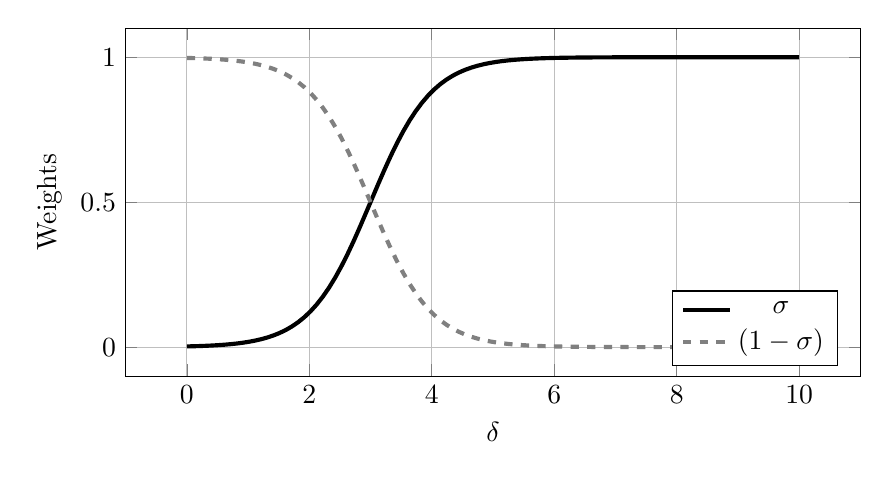
\begin{tikzpicture}%[trim axis left]
		\begin{axis}[
		  width = 0.9\textwidth,
		  height = 6cm,
		  domain = 0.001:10,
		  samples = 100,
		  grid = both,
		  xlabel = $\delta$,
		  ylabel = Weights,
		  legend pos = south east] % customize the axis environment with whatever you want (xmax,ymin,...)	  
		\addplot [color=black, solid, line width=1.5pt] {0.5*tanh(x-3)+0.5}; \addlegendentry{$\sigma$};
		\addplot [color=gray, dashed, line width=1.5pt] {1-(0.5*tanh(x-3)+0.5)}; \addlegendentry{$(1-\sigma)$};
		\end{axis}
	\end{tikzpicture}
	\caption{Plot with Tikz (without detour via Matlab)}
\end{figure}


\begin{figure}[htb]
	% Define block styles
	\tikzstyle{decision} = [diamond, draw, %fill=green!20, 
		text width=4.0em, text badly centered, node distance=2cm, inner sep=0pt]
	\tikzstyle{block} = [rectangle, draw, %fill=green!20, 
	text width=5em, text centered, rounded corners, minimum height=2em]
	\tikzstyle{line} = [draw, -latex']
	\tikzstyle{cloud} = [draw, ellipse, %fill=orange!40,
				 node distance=3cm, minimum height=2em]
	
	\begin{center}
		\begin{tikzpicture}[node distance = 1.4cm, auto, every node/.style={font=\sffamily\scriptsize}]
		% Place nodes
		\node [block] (init) {initialize model};
		\node [cloud, left of=init] (expert) {expert};
		\node [cloud, right of=init] (system) {system};
		\node [block, below of=init] (identify) {identify candidate models};
		\node [block, below of=identify] (evaluate) {evaluate candidate models};
		\node [block, left of=evaluate, node distance=3cm] (update) {update model};
		\node [decision, below of=evaluate] (decide) {is best candidate better?};
		\node [block, below of=decide, node distance=1.9cm] (stop) {stop};
		% Draw edges
		\path [line] (init) -- (identify);
		\path [line] (identify) -- (evaluate);
		\path [line] (evaluate) -- (decide);
		\path [line] (decide) -| node [near start] {yes} (update);
		\path [line] (update) |- (identify);
		\path [line] (decide) -- node {no}(stop);
		\path [line,dashed] (expert) -- (init);
		\path [line,dashed] (system) -- (init);
		\path [line,dashed] (system) |- (evaluate);
		\end{tikzpicture}
	\end{center}
	\caption{Flowchart with Tikz}
\end{figure}